\chapter{Implementation} \label{implementation}
\textmd{In diesem Kapitel wird die Implementation des Partikelsystems aus dem Projekt erl�utert. Dabei wird auf die Techniken eingegangen, die zur Realisierung des Partikelsystems eingesetzt wurden.}

\section{Datenstrukturen} \label{datastructures}
\textmd{Dieser Abschnitt beschreibt die angelegten Datenstrukturen und Algorithmen um Partikelsysteme zu realisieren und zu verwalten. Davon abgegrenzt ist die Darstellung die in Abschnitt \ref{rendering} beschrieben wird.}

\textmd{\\Partikel wurden mit der Klasse Particle modelliert. Sie verf�gt �ber eine Lebenszeit, physikalische Eigenschaften wie Position, Geschwindigkeit und Beschleunigung, sowie Farbe. Eine update-Funktion sorgt f�r das Aktualisieren der Eigenschaften �ber den Lebenszyklus des Partikels. Getter und Setter erm�glichen den Zugriff auf ihre Eigenschaften, wobei die Setter eher nicht direkt verwendet werden sollten. F�r das Setzen der Eigenschaften gibt es mit Particle.Builder eine Klasse �ber die Partikel konfiguriert und anschlie�end erzeugt werden k�nnen.}

\textmd{\\Partikelsysteme sind durch die Klasse ParticleSystem modelliert. Ein Partikelsystem verwaltet alle seine zugeh�rigen Partikel und erh�lt bei der Instanziierung einen Particle.Builder �bergeben, anhand dessen Konfiguration er seine Partikel erzeugt.}
\textmd{\\Das Partikelsystem hat eine update-Methode, die das Erzeugen neuer Partikel sowie das Aktualisieren und Sterben bestehender Partikel umsetzt. Daf�r wird anhand der Systemzeit berechnet wie viele Millisekunden seit dem letzten update-Aufruf vergangen sind und als zeitliches Delta verwendet.}
\textmd{\\An einem Partikelsystem kann festgelegt werden, wie viele Partikel maximal gleichzeitig existieren und wie viele Partikel pro Sekunde erzeugt werden k�nnen. Um einen stetigen Partikelfluss zu gew�hrleisten hat sich die Faustregel in Formel \ref{emissionrate} durchgesetzt, vgl. \cite[Abschnitt Emission Rate]{greer2012}.}
\begin{align}
	Emissionsrate = \frac{maxPartikel}{Lebenszeit_{Partikel}}
	\label{emissionrate}
\end{align}

\textmd{\\}

\textmd{\\TODO: ParticleSystemManager erkl�ren}

\section{Lebenszyklusmanagement} \label{lifecyclemanagement}
\textmd{Partikelsysteme erzeugen st�ndig neue Partikel und bestehende Partikel sterben. }

\textmd{\\TODO: ParticleSystemManager, Particle-Pool erkl�ren }
\cite{gamasutra2000} (ParticleSystemManager)
\cite{greer2012}, \cite{natureofcode2012}, \cite{khan} (Particle-Pool)

\section{Kr�fte} \label{forces}
\textmd{}

\textmd{\\TODO: Kr�fte, Attraktoren und Repeller}
\cite{natureofcode2012} \cite{khan}

\section{Darstellung} \label{rendering}
\textmd{In diesem Abschnitt wird die Darstellung der Partikelsysteme beschrieben. Das Projekt verwendet den aus dem Praktikum bekannten Szenengraphen. Die Einbindung eines Partikelsystems in den Szenengraphen wird mit einem ParticleSystemNode realisiert. Dieser erh�lt bei seiner Erzeugung das Partikelsystem das er darstellen soll. Ab der Einbindung in den Szenengraphen ist der ParticleSystemNode f�r das Aktualisieren und Zeichnen des Partikelsystems zust�ndig. Zum Zeichnen wird ein VertexBufferObject der einzelnen Partikel erzeugt und OpenGL �bergeben. Zur fl�ssigen Darstellung des Partikelsystems geschieht das in jedem Renderzyklus. Um die H�ufigkeit des Renderzyklus festzulegen, kann �ber die Klasse ParticleSystemShowcaseScene eine gew�nschte Frames-Per-Second-Rate angegeben werden.}

\textmd{\\Die einzelnen Partikel werden als einfache, farbige Punkte gezeichnet. Sie k�nnen �ber die Zeit ausgeblendet werden, was in OpenGL zu Problemen mit der Transparenz f�hrt. Der n�chste Abschnitt beschreibt das Problem und den Umgang mit der Transparenz in OpenGL.}

\section{Transparenz} \label{transparency}
\textmd{Dieser Abschnitt behandelt den Umgang mit Transparenz in der Darstellung der einzelnen Partikel. Standardm��ig werden die Partikel ohne eine bestimmte Sortierung gezeichnet. Das sorgt in OpenGL daf�r, dass Transparenz nicht richtig dargestellt werden kann. Wenn ein transparentes Objekt das n�her zur Kamera ist zuerst gezeichnet wird und danach eines das weiter hinten ist, so werden die Pixel des ersten Objekts nicht mehr angepasst. F�r ein Partikelsystem mit Transparenz sieht das aus wie in Abbildung \ref{transparency-no-btf}. In der Abbildung k�nnen dunkle Partikel beobachtet werden, die transparent sein sollten.}
\begin{figure}[h]
	\begin{center}
		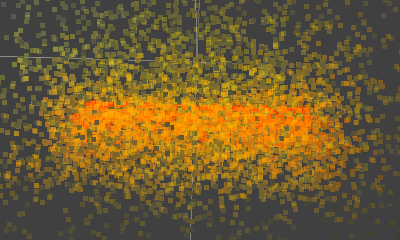
\includegraphics[width=25em]{img/transparency_no_back-to-front_ordering.png}
		\caption{Partikelsystem ohne Back-to-Front-Sortierung}
		\label{transparency-no-btf}
	\end{center}
\end{figure}
\textmd{\\Um die Transparenz korrekt darzustellen wurde eine Back-to-Front-Sortierung unter Zuhilfenahme der Binary-Space-Partition berechnet. Bei der Binary-Space-Partition werden die Partikel r�umlich durch Hyperebenen in einer Baumstruktur getrennt, vgl. \cite[Folie 26]{jenke2016}. Jeder Partikel befindet sich dann entweder vor oder hinter einer Hyperebene, bei der er einsortiert wurde. Betrachtet man nun einen Sichtpunkt, so kann anhand der Hyperebenen die Back-to-Front-Sortierung ermittelt werden, vgl. \cite[Folie 32]{jenke2016}.}
\textmd{\\Die Back-to-Front-Sortierung wiederum ist wichtig um die Partikel in der richtigen Reihenfolge zu zeichnen, sodass OpenGL die Transparenz korrekt darstellt. In der Darstellung des Beispiels aus Abbildung \ref{transparency-no-btf} mit Back-to-Front-Sortierung (siehe Abbildung \ref{transparency-with-btf}) fallen nun keine dunklen Partikel mehr auf.}
\begin{figure}[h]
	\begin{center}
		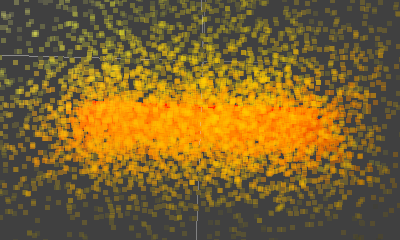
\includegraphics[width=25em]{img/transparency_with_back-to-front_ordering.png}
		\caption{Partikelsystem mit Back-to-Front-Sortierung}
		\label{transparency-with-btf}
	\end{center}
\end{figure}
\textmd{\\\\Es sollte erw�hnt werden, dass die Back-to-Front-Sortierung insbesondere bei einer gro�en Anzahl von Partikeln gewisse Performance-Einbu�en mit sich f�hrt. W�hrend ein Partikelsystem mit 10.000 Partikeln ohne Back-to-Front-Sortierung in meinen Tests mit einer Bildrate von 30 Frames-per-Second gerendert werden kann, so f�llt die Bildrate mit Back-to-Front-Sortierung in dem Szenario auf 10 Frames-per-Second.}